%%% Local Variables: 
%%% mode: latex
%%% TeX-master: "../master.tex"
%%% LaTeX-command: "latex -shell-escape"
%%% End:

\chapter{Union-Find}
%=================================================================================================================================================

\section{Dynamic Connectivity}
\subsection{Applications involve manipulating objects of all types}
\begin{itemize}
 \item Pixels in a digital photo
 \item Computers in a network
 \item Friends in a social network.
 \item Transistors in a computer chip
 \item Variable name in Fortran program
 \item Metallic sites in a composite system
\end{itemize}

\vspace{10 mm}

\textbf{Given a set of N objects}
\begin{description}
  \item[Union command:] connect two objects
  \item[Find/connected query:] is there a path connecting the two objects?
\end{description}

\begin{figure}[h]
   \centering
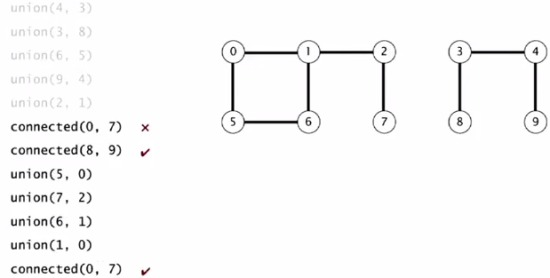
\includegraphics[scale=0.4]{tex_files/images/dynamicconnectivity.jpg}
\end{figure}



\vspace{10 mm}

\subsection{Implementing the operations}
\begin{description}
  \item[Find Query] Check if two objects are in the same component.
  \item[Union Command] Replace components containing two objects with their union.
\end{description}
For example if you have [0][1 4 5][2 3 6 7] where each [X...X] represents the connectec components if you use the operation \textbf{union(2,5)}
you will have [0][1 2 3 4 5 6 7]


\subsection{Union-find data type (API)}

\textbf{Goal} Design efficient data structure for union-find.
\begin{itemize}
\item Number of objects N can be huge.
\item Number of operations M can be huge.
\item Find queries and union commands may be intermixed.
\end{itemize}


\begin{table}[h]
\begin{center}
\begin{tabular}{cc}
\textbf{Public Class UF}        & \multicolumn{1}{l}{}                                          \\ \hline
UF(int N)                       & initialize union-find data structure with N objects(0 to N-1) \\ \hline
void union( int p, int q)       & add connection between p and q                                \\ \hline
boolean connected(int p, int q) & are p and q in the same component ?                           \\ \hline
int find(int p)                 & component identifier for p(0 to N-1)                          \\ \hline
int count()                     & number of components                                          \\ \hline
\end{tabular}
\end{center}
\end{table}

%=================================================================================================================================================
\section{Quick Find}
%=================================================================================================================================================

\textbf{Data Structure}
\begin{itemize}
\item Integer array id[] of size N.
\item Interpretation: p and q are connected if they have the same id.
\end{itemize}


\textbf{Find} Check if p and q have the same id.
\textbf{Union} to merge componenets containing p and q, change all entries whose id equals to id[p] to id[q]

\begin{minted}
[
frame=lines,
framesep=2mm,
baselinestretch=1.2,
fontsize=\footnotesize,
linenos
]{java}
public class QuickFind
{
        private int[] id;

        public QuickFind(int N)
        {
                id= new int[N];
                for ( int i = 0; i < N; i++)
                        id[i] = i;
        }
        
        public boolean find(int p, int q)
        {
                return id[p] == id[q];
        }
        
        public void unite(int p, int q)
        {
                int pid = id[p];
                for (int i=0; i< id.length; i++)
                        if (id[i] == pid) id[i] = id[q];
        }
}

\end{minted}

\textbf{Cost Model} Number of array acesses for read or write.

\begin{table}[h]
\centering
\begin{tabular}{clll}
\hline
\multicolumn{1}{|c|}{\textbf{Algorithm}} & \multicolumn{1}{l|}{\textbf{initialize}} & \multicolumn{1}{l|}{\textbf{union}} & \multicolumn{1}{l|}{\textbf{find}} \\ \hline
Quick-Find                               & N                                        & N                                   & \multicolumn{1}{c}{1}             
\end{tabular}
\end{table}

\textbf{ex.} takes $N^2$ array acesses to process a sequence of N union commands on N objects.


%=================================================================================================================================================
\section{Quick Union}
%=================================================================================================================================================

\begin{minted}
[
frame=lines,
framesep=2mm,
baselinestretch=1.2,
fontsize=\footnotesize,
linenos
]{java}
public class QuickUnionUF
{
  private int[] id;
   
  public QuickUnionUF(int N)
  {
    id = new int[N];
    for (int i = 0; i < N; i++) id[i] = i;
  }
  
  private int root(int i)
  {
    while(i != id[i]) i = id[i];
    return i;
  }
  
  public bolean connected(int p, int q)
  {
    return root(p) == root(q);
  }
  
  public void union(int p, int q)
  {
    int i = root(p);
    int j = root(q);
    int[i] = j;
  }
}
\end{minted}

\begin{table}[h]
\centering
\begin{tabular}{clll}
\hline
\multicolumn{1}{|c|}{\textbf{Algorithm}} & \multicolumn{1}{l|}{\textbf{initialize}} & \multicolumn{1}{l|}{\textbf{union}} & \multicolumn{1}{l|}{\textbf{find}} \\ \hline
Quick-Find                               & N                                        & N                                   & \multicolumn{1}{c}{1}   \\ \hline
Quick-Union                              & N                                        & N                                   & N          
\end{tabular}
\end{table}

\textbf{Quick-Find defect}
\begin{itemize}
\item Union too expensive (N array acesses).
\item Trees are flat, but too expensive to keep them flat.
\end{itemize}

\textbf{Quick-Union defect}
\begin{itemize}
\item Trees can get tall.
\item Find too expensive ( could be N array accesses).
\end{itemize}

\subsection{improvements}
